%% =====================================================================
%% Paper (doble columna): SIGRET-AQP — soporte a la decisión para
%% localizar minimarkets independientes en Arequipa Metropolitana
%% Compilar con:  tectonic main.tex      (o pdflatex dos veces)
%% Las referencias están escritas a mano en estilo APA 7 (sección final).
%% =====================================================================
\documentclass[10pt,letterpaper,twocolumn]{article}

\usepackage[utf8]{inputenc}
\usepackage[T1]{fontenc}
\usepackage{mathptmx}
\usepackage[spanish,es-nodecimaldot,es-tabla]{babel}
\usepackage[top=0.8in,bottom=0.85in,left=0.75in,right=0.75in,columnsep=0.25in]{geometry}
\usepackage{amsmath}
\usepackage{booktabs}
\usepackage{graphicx}
\usepackage{caption}
\usepackage[hyphens]{url}
\usepackage[hidelinks,colorlinks=true,linkcolor=black,citecolor=black,urlcolor=blue]{hyperref}
\usepackage[round,authoryear]{natbib}
\usepackage{microtype}
\usepackage{array}
\usepackage{balance}

\setlength{\parindent}{0.9em}
\setlength{\parskip}{0pt}
\setlength{\emergencystretch}{1.5em}
\Urlmuskip=0mu plus 2mu
\captionsetup{font=small,labelfont=bf,labelsep=period,skip=4pt}
\setlength{\bibsep}{2pt}
\bibpunct[, ]{(}{)}{;}{a}{}{,}
\setlength{\textfloatsep}{8pt plus 2pt minus 2pt}
\setlength{\floatsep}{8pt plus 2pt minus 2pt}
\setlength{\intextsep}{8pt plus 2pt minus 2pt}

\begin{document}

%% ---------------------------------------------------------------------
\twocolumn[{%

\begin{center}
{\LARGE\bfseries Sistema de soporte a la decisión basado en analítica geoespacial y aprendizaje automático para la localización de minimarkets independientes en Arequipa Metropolitana}\\[1.1em]
{\large Fernando Gabriel Casapía Loayza\,$^{1}$ \quad Paolo Marcelo Rivera Salas\,$^{1}$ \quad Karina Rosas Paredes\,$^{1}$}\\[0.5em]
{\small $^{1}$Escuela Profesional de Ingeniería de Sistemas, Universidad Católica de Santa María, Arequipa, Perú}\\[0.3em]
{\small \texttt{fernando.casapia@estudiante.ucsm.edu.pe} \quad \texttt{paolo.rivera@estudiante.ucsm.edu.pe} \quad \texttt{kparedes@ucsm.edu.pe}}\\[0.3em]
{\footnotesize ORCID: 0009-0001-3899-1474 \quad 0009-0004-2718-3780 \quad 0000-0003-4650-7432}
\end{center}
\vspace{0.4em}
\begin{center}
\begin{minipage}{0.94\textwidth}
\small
\noindent\textbf{Resumen.}
La elevada mortalidad empresarial del comercio minorista en Arequipa, con 4\,797 altas y 4\,720 bajas de empresas en el tercer trimestre de 2024, y la falta de herramientas objetivas de localización para el comerciante independiente motivaron esta investigación, cuyo objetivo fue desarrollar y validar un sistema de soporte a la decisión, basado en analítica geoespacial y aprendizaje automático, para priorizar ubicaciones de minimarkets independientes en Arequipa Metropolitana. Con la metodología Design Science Research se construyó una malla de 3\,717 celdas H3 que integra el Censo 2017, OpenStreetMap y el localizador de una cadena de descuento duro (127 aperturas fechadas con Internet Archive). Ante la ausencia de datos de ventas, la variable objetivo se definió por preferencia revelada. Se compararon regresión logística, Random Forest, XGBoost y un ensamble sobre 37 predictores, mediante validación cruzada espacial y backtesting contra las 39 aperturas de 2025 y 2026. El ensamble alcanzó un ROC-AUC de 0,917 en validación espacial (0,766 en celdas viables) y 0,809 en backtesting, con un lift de 4,91 en el decil superior (IC 95\,\%: 3,02--6,22); su ventaja sobre el mejor criterio univariado (58,3\,\%) no fue significativa. La usabilidad promedió 77,83 en la escala SUS y la aceptación 4,13 sobre 5, aunque los propietarios de minimarket puntuaron por debajo del umbral (SUS 74,00; TAM 3,90). La hipótesis se sostiene según los criterios preestablecidos, con una capacidad moderada de discriminación entre ubicaciones comparables.

\smallskip
\noindent\textit{Palabras clave:} localización comercial, analítica geoespacial, aprendizaje automático

\medskip
\noindent\textbf{Abstract.}
The high business mortality of Arequipa's retail sector (4,797 business registrations and 4,720 closures in the third quarter of 2024) and the lack of objective site-selection tools for independent merchants motivated this research, whose objective was to develop and validate a decision support system, based on geospatial analytics and machine learning, to prioritize locations for independent minimarkets in Metropolitan Arequipa. Using Design Science Research, a grid of 3,717 H3 cells was built, integrating the 2017 Census, OpenStreetMap, and the store locator of a hard-discount chain (127 openings dated with Internet Archive). In the absence of sales data, the target variable was defined by revealed preference. Logistic regression, Random Forest, XGBoost, and an ensemble were compared on 37 predictors using spatial cross-validation and a backtest against the 39 openings of 2025 and 2026. The ensemble reached a ROC-AUC of 0.917 under spatial validation (0.766 on viable cells) and 0.809 in the backtest, with a lift of 4.91 in the top decile (95\% CI: 3.02--6.22); its advantage over the best univariate criterion (58.3\%) was not significant. Usability averaged 77.83 on the SUS scale and acceptance 4.13 out of 5, although minimarket owners scored below the threshold (SUS 74.00; TAM 3.90). The hypothesis is supported under the pre-established criteria, with a moderate ability to discriminate between comparable locations.

\smallskip
\noindent\textit{Keywords:} commercial site selection, geospatial analytics, machine learning
\end{minipage}
\end{center}
\vspace{0.8em}
}]

%% ---------------------------------------------------------------------
\section{Introducción}

En el Perú existían 3\,409\,102 empresas activas al tercer trimestre de 2024, con una mortalidad (2,56\,\%) superior a la natalidad (2,31\,\%); más de la mitad de las altas del sector comercio corresponde al comercio de alimentos, el perfil de la bodega y del minimarket de barrio \citep{inei2024}. El Ministerio de la Producción contabiliza más de 380\,000 bodegas formales, que generan S/\,912 millones de valor agregado y 879\,910 empleos \citep{produce2025}, frente a un retail moderno que supera los 1\,570 locales Mass (localizador de la cadena, julio de 2026) y los 780 Tambo \citep{peruretail2026}; el \textit{hard discount} avanza en la región (21\,\% del supermercadismo en Colombia, 30,5\,\% del retail moderno en México y 11\,\% en el Perú; \citealp{deloitte2025}). En ese contexto, Arequipa fue en el tercer trimestre de 2024 el segundo departamento con más altas (4\,797) y más bajas (4\,720) empresariales, casi un negocio cerrado por cada uno abierto \citep{inei2024}.

La decisión de dónde ubicar un establecimiento es un problema clásico del retail \citep{huff1964}. La disponibilidad de datos la trasladó al aprendizaje automático: la densidad y el tipo de comercio vecino predicen la popularidad de una tienda \citep{karamshuk2013}, la movilidad urbana anticipa su fracaso \citep{dsilva2018}, y ensambles y XGBoost alcanzan exactitudes de 0,75 a 0,92 \citep{lu2024,zhao2025,ou2026}. Sin embargo, esas soluciones dependen de insumos privados, como series de ventas por local \citep{lu2024,hu2025} o señalización de telefonía móvil \citep{zou2024}, que un comerciante independiente no puede obtener. Hasta donde alcanza la revisión realizada, en el Perú no se ha reportado un modelo que aprenda de aperturas históricas para la localización comercial (véase, para Lima, \citealp{rossi2024}).

A ello se suma un problema de validación: la autocorrelación espacial infla el desempeño estimado cuando las particiones de entrenamiento y prueba son aleatorias \citep{ploton2020,roberts2017,meyer2021}; para la región de Arequipa se ha documentado un sesgo de entre 6\,\% y 18\,\% \citep{kumar2025}.

Este trabajo presenta SIGRET-AQP, un sistema de soporte a la decisión construido íntegramente con fuentes públicas, y reporta su validación. Las contribuciones son: (i) un repositorio geoespacial abierto de 3\,717 celdas hexagonales con 49 variables; (ii) una variable objetivo por preferencia revelada \citep{samuelson1938}, a partir de las aperturas de una cadena con equipo profesional de geomarketing; (iii) una validación espacial y temporal que incluye la detección y corrección de una fuga de información; y (iv) una aplicación web evaluada con quince usuarios. La hipótesis, fijada antes de los experimentos, es que el sistema prioriza ubicaciones con una capacidad discriminativa superior a la de criterios univariados de referencia: ROC-AUC mayor que 0,85 bajo validación cruzada espacial en bloques, y, en el backtesting temporal, un lift en el decil superior mayor o igual que 3 y superior al del mejor criterio univariado.

%% ---------------------------------------------------------------------
\section{Materiales y métodos}

\subsection{Diseño y unidad de análisis}

Se siguió la metodología Design Science Research \citep{peffers2007}. El área de estudio comprende los diecisiete distritos de Arequipa Metropolitana ($\approx$433\,km$^2$). El territorio se discretizó en celdas H3 de resolución~9 \citep{brodsky2018,kmoch2022}, más un anillo de vecindad de orden uno que cubre la expansión urbana posterior a 2017: 3\,717 celdas de $\approx$0,11\,km$^2$ (2\,597 del núcleo censado y 1\,120 del anillo). La población censal se transfirió de la manzana a la celda por ponderación areal, sin pérdida ni duplicación. Se reconoce la sensibilidad de los resultados a la zonificación \citep{openshaw1984}.

\subsection{Fuentes de datos}

La Tabla~\ref{tab:fuentes} resume las fuentes, todas de acceso público y con licencia que permite su almacenamiento y redistribución. La red histórica de competencia se reconstruyó comparando cuatro versiones archivadas del localizador (2024 a 2026): cada tienda se fechó con el primer año en que aparece, tras normalizar su código. Resultaron 127 tiendas, 86 existentes al corte de 2024, 32 aperturas en 2025 y 9 en 2026. El Padrón Reducido del RUC se evaluó y se descartó como predictor: tras depurar las formas legales solo 212 de 5\,124 registros resultaron identificables como bodega.

\begin{table}[t]
\centering
\caption{Fuentes de datos del sistema.}
\label{tab:fuentes}
\footnotesize
\setlength{\tabcolsep}{3pt}
\begin{tabular}{>{\raggedright\arraybackslash}p{2.1cm}>{\raggedright\arraybackslash}p{3.0cm}>{\raggedright\arraybackslash}p{2.5cm}}
\toprule
Fuente & Contenido utilizado & Uso \\
\midrule
Censo Nacional 2017 \citep{inei2018} & 21\,705 manzanas, 1\,018\,031 habitantes & Demanda poblacional \\
OpenStreetMap (ODbL) & 182 comercios (169 sin cadenas), 3\,072 POIs, red vial & Competencia, POIs, morfología \\
Localizador de la cadena & 127 tiendas con coordenadas & Variable objetivo \\
Internet Archive & 4 versiones del localizador (2024--2026) & Fechado de aperturas \\
\bottomrule
\end{tabular}
\end{table}

\subsection{Variable objetivo y predictores}

Ante la ausencia de datos de ventas, una celda se etiquetó como positiva si la cadena decidió abrir en ella (preferencia revelada); la tasa base es de 3,3\,\%. Se construyeron 49 variables en cinco familias: demanda poblacional en anillos de vecindad ($k=1,2,3$), estructura territorial, morfología vial, puntos de interés generadores de flujo (nueve categorías) y competencia observada. Se excluyó toda variable derivada de la red de la cadena (12 variables), lo que dejó 37 predictores efectivos (Sección~\ref{sec:fuga}).

\subsection{Modelos}

Se compararon cuatro modelos (Figura~\ref{fig:flujo}): regresión logística con regularización L2 ($C=0{,}5$) y estandarización previa; Random Forest \citep{breiman2001} con 800 árboles, \texttt{min\_samples\_leaf}$=5$ y $\sqrt{p}$ atributos por división; XGBoost \citep{chen2016} con 400 árboles, profundidad 3, tasa de aprendizaje 0,05, submuestreo 0,8, $\lambda=3$ y \texttt{scale\_pos\_weight} igual a la razón de clases; y un ensamble por promedio de rangos percentiles. Los tres modelos base ponderan las clases de forma inversamente proporcional a su frecuencia \citep{he2009}.

\begin{figure}[t]
\centering
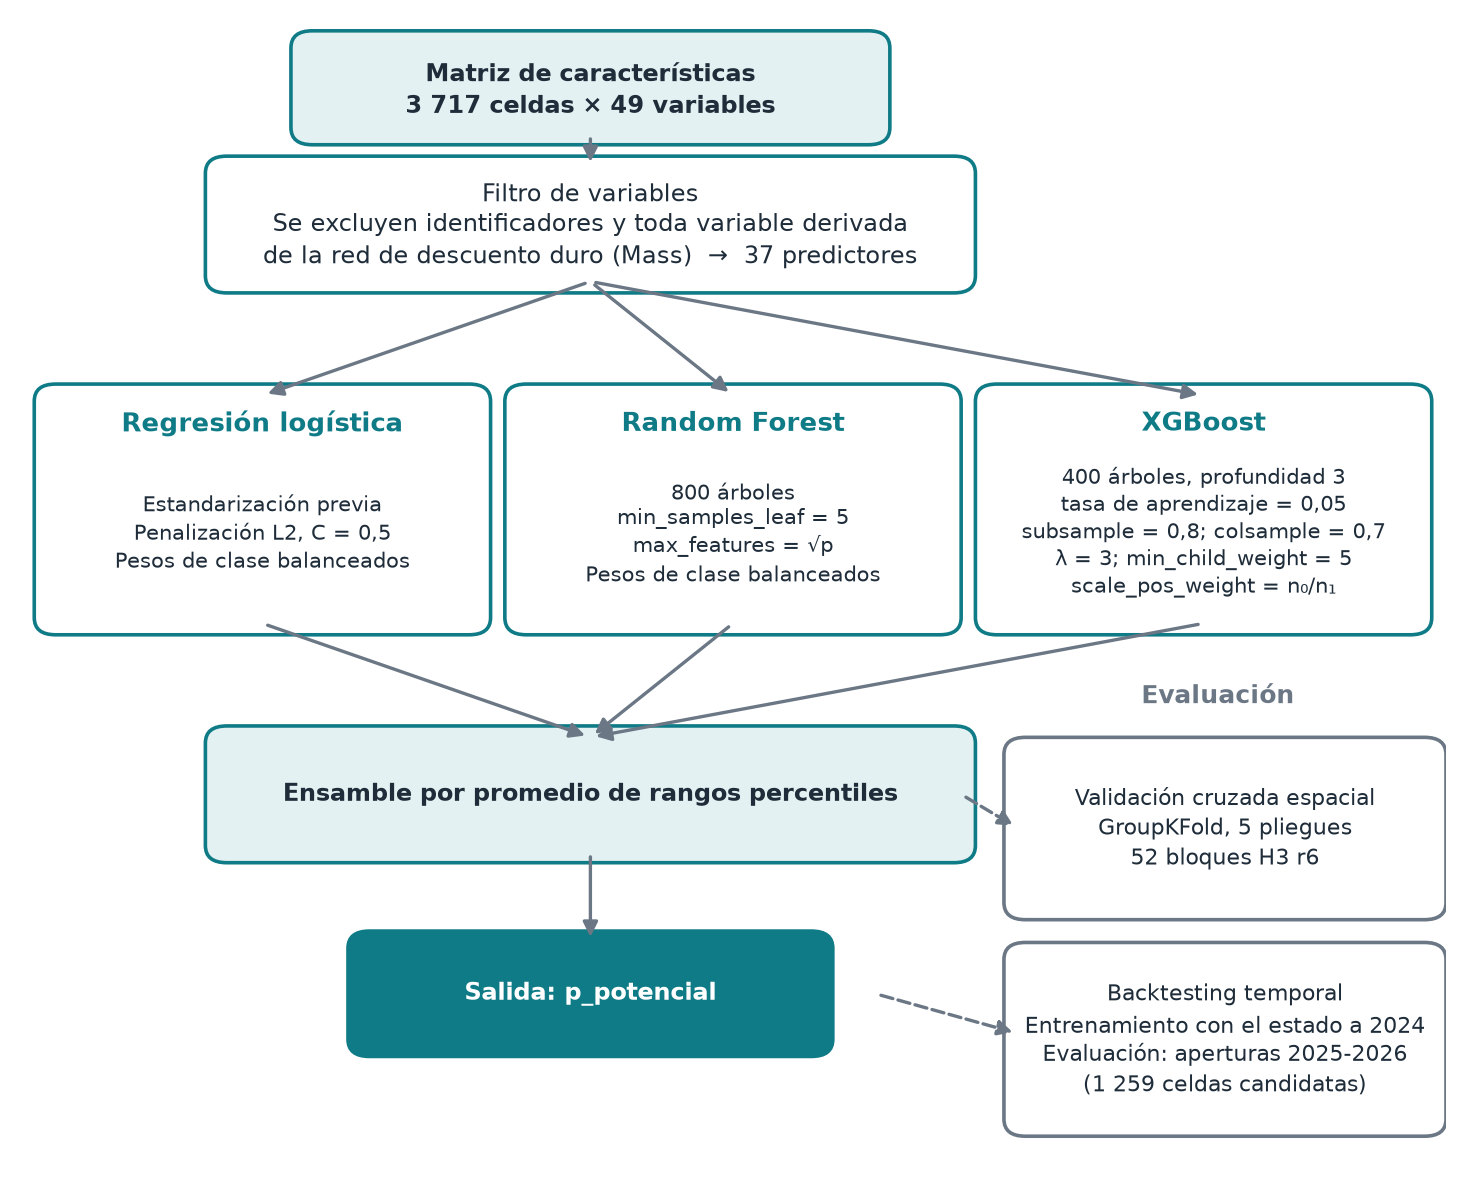
\includegraphics[width=\linewidth]{figuras/fig_flujo_modelado.png}
\caption{Flujo de modelado y evaluación. Fuente: elaboración propia.}
\label{fig:flujo}
\end{figure}

\subsection{Validación}

\textbf{Validación cruzada espacial.} Cada celda se agrupó por su hexágono padre de resolución~6 (52 bloques) y se aplicó una validación cruzada agrupada de cinco pliegues, con el estandarizador ajustado solo sobre el subconjunto de entrenamiento. Además del ROC-AUC y el PR-AUC sobre las 3\,717 celdas, se calculó el ROC-AUC restringido a las 1\,341 celdas \textit{viables} (con al menos 1\,500 habitantes alcanzables en su anillo de vecindad), que son las que el sistema ordena.

\textbf{Backtesting temporal.} Los modelos se entrenaron con el estado de la red al corte de 2024 y se evaluaron sobre las 1\,259 celdas candidatas (viables y sin la cadena en 2024), contra las 39 aperturas ocurridas en 2025 y 2026 (tasa base de 3,10\,\%). Los predictores se calcularon con las capas de OpenStreetMap al 31 de diciembre de 2024 y se excluyeron los locales de la cadena. Se reportan ROC-AUC, PR-AUC, el lift en el decil superior (125 celdas) y los aciertos entre las 20 primeras. Se incorporaron tres líneas base univariadas (densidad poblacional, población alcanzable y densidad de puntos de interés) e intervalos de confianza por \textit{bootstrap} de 1\,000 remuestreos. Para medir la sensibilidad a la inicialización, los modelos con componente aleatorio (Random Forest y XGBoost) se repitieron con diez semillas; se reporta la media y la desviación estándar.

\subsection{Score de decisión y simulación económica}

El ranking combina el perfil aprendido con la demanda residual y penaliza la cercanía de la cadena:
\begin{equation}
S_i=\bigl[w\,\hat p_i+(1-w)\,\tilde d_i\bigr]\bigl(1-\pi\,r_i\bigr),
\end{equation}
\begin{equation}
r_i=\max\!\Bigl(0,\,1-\tfrac{\text{dist}_i}{R}\Bigr),
\end{equation}
donde $\hat p_i$ es la probabilidad del ensamble (rango percentil), $\tilde d_i$ es el rango percentil de la demanda residual $d_i=\text{pob}_{k1,i}\cdot 180/(1+o_i)$, $o_i$ es la oferta rival (competencia de OpenStreetMap más tres veces las tiendas de la cadena en el anillo), $\text{dist}_i$ es la distancia a la tienda de la cadena más próxima y $R$ es el radio de amenaza. El score es cero para las celdas no viables.

Un simulador económico, derivado del modelo de interacción espacial de \citet{huff1964} con exponente de atractividad fijado en la unidad (limitación señalada por \citealp{liang2020}), estima la cuota de mercado, las ventas mensuales, el margen bruto y el periodo de recuperación de la inversión. Como la cobertura de comercios en OpenStreetMap es mínima, la oferta informal se estima a partir de la densidad poblacional (una bodega por cada 120 habitantes) y se toma el máximo frente al conteo observado. El usuario ajusta nueve parámetros (peso del perfil, penalización, radio de amenaza, población mínima, gasto per cápita de S/\,180, habitantes por bodega, superficie de venta de 100\,m$^2$, inversión de S/\,160\,000 y margen bruto de 22\,\%).

\subsection{Elicitación de pesos y sensibilidad del ranking}

Los parámetros del score se derivaron del Proceso Analítico Jerárquico \citep{saaty1990} aplicado a diez propietarios de minimarket, con matrices de comparación pareada sobre cuatro criterios (demanda alcanzable, perfil de sitio, competencia instalada y amenaza del retail moderno), media geométrica del panel y razón de consistencia menor que 0,10. El radio de amenaza se obtuvo de forma directa, como la mediana de la distancia a partir de la cual el propietario deja de preocuparse por la competencia. La estabilidad del ranking se evaluó variando $\pm$20\,\% los cuatro parámetros del score, con un criterio de aceptación de permanencia del 70\,\% del Top-10.

\subsection{Aplicación web y evaluación con usuarios}

El pipeline en Python genera cuatro archivos JSON (569\,KB en total) que una aplicación web (Vue~3, Vuetify y MapLibre GL, servida con Laravel) consume en el navegador sin backend de cómputo. Tiene seis vistas: resumen, mapa de oportunidad, ranking, simulador de apertura, validación y fuentes, y el recálculo del score al mover un control toma menos de 10\,ms. Las Figuras~\ref{fig:vistas} y~\ref{fig:app} muestran las vistas principales y la de fuentes. La aplicación fue evaluada por 15 usuarios (5 propietarios de minimarket, 4 corredores inmobiliarios, 3 docentes y 3 estudiantes de posgrado) con la Escala de Usabilidad del Sistema \citep[SUS;][]{brooke1996} y el Modelo de Aceptación de la Tecnología \citep[TAM;][]{davis1989}. Los criterios de aceptación fueron SUS~$\geq 75$ y TAM~$\geq 4{,}0$. El tamaño de la muestra se sustenta en \citet{tullis2004}.

\begin{figure*}[t]
\centering
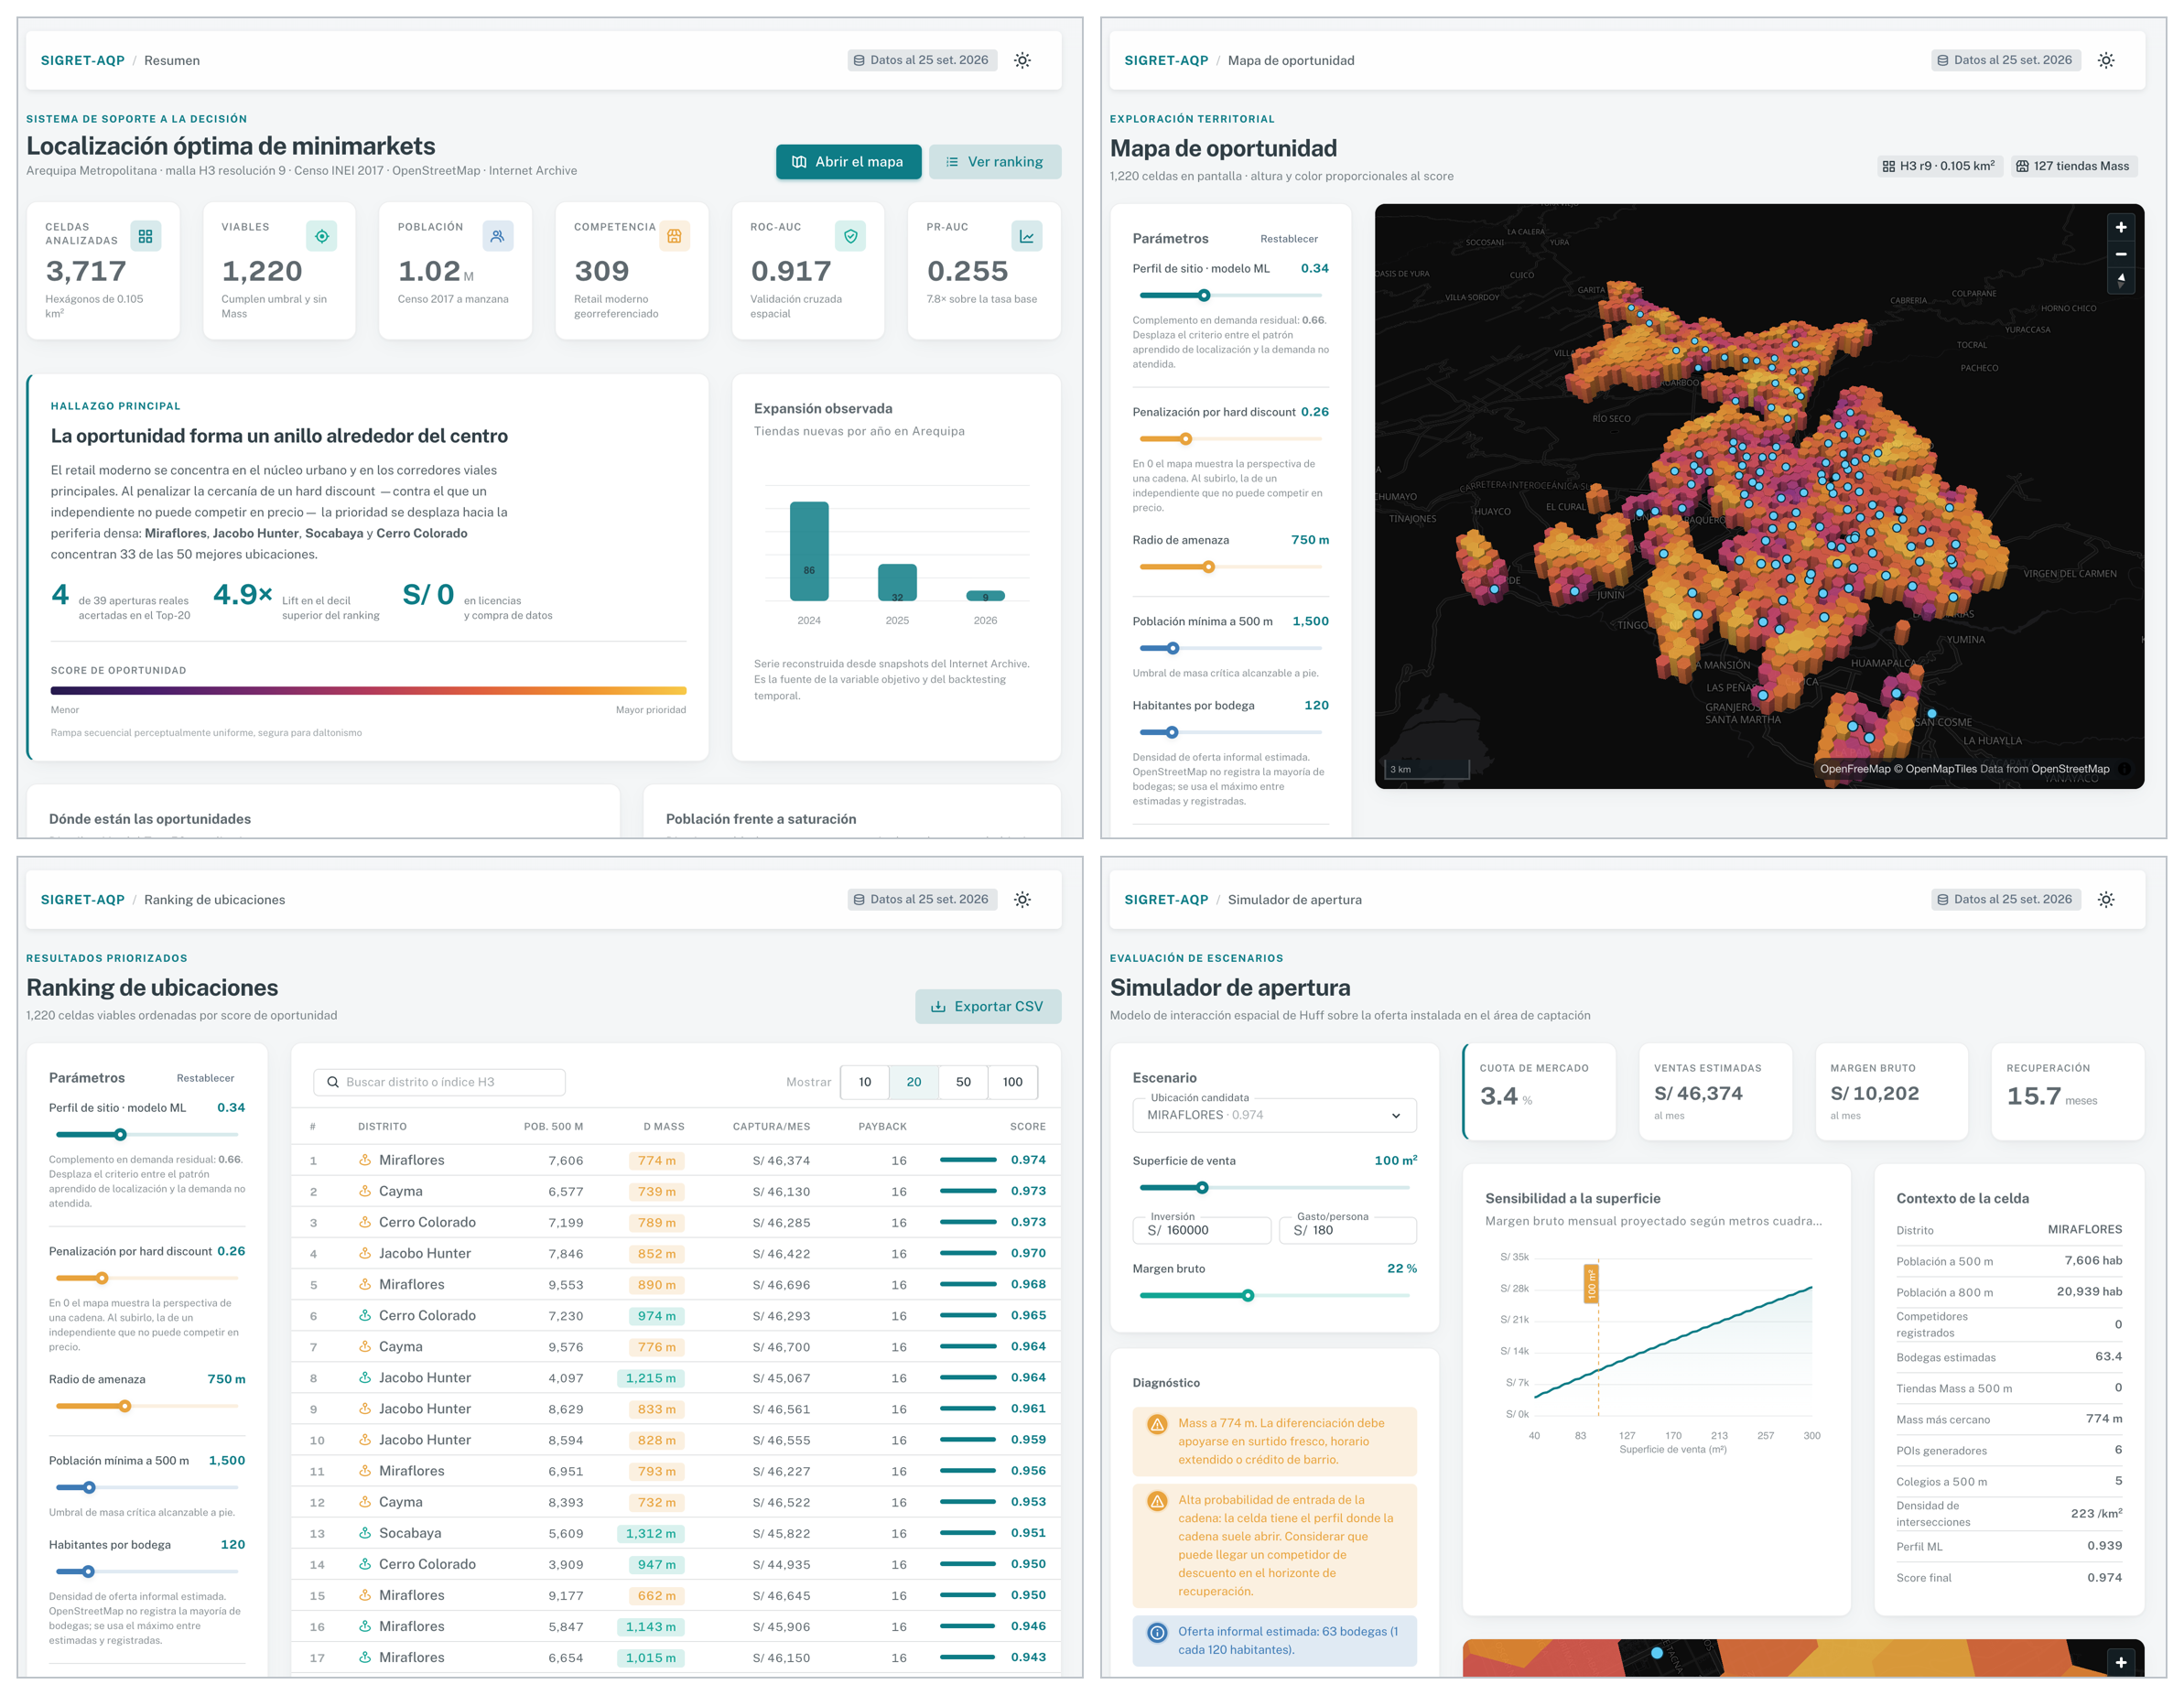
\includegraphics[width=0.78\textwidth]{figuras/fig_app_vistas.png}
\caption{Vistas principales de la aplicación SIGRET-AQP: resumen con los indicadores de validación (arriba a la izquierda), mapa de oportunidad en 3D con los parámetros del score (arriba a la derecha), ranking de ubicaciones (abajo a la izquierda) y simulador de apertura (abajo a la derecha). Fuente: capturas de la aplicación.}
\label{fig:vistas}
\end{figure*}

\begin{figure}[t]
\centering

\includegraphics[width=\linewidth]{figuras/fig_fuentes.png}
\caption{Vista \textit{Fuentes de datos} de la aplicación: procedencia de cada fuente y arquitectura del procesamiento. Fuente: captura de la aplicación SIGRET-AQP.}
\label{fig:app}
\end{figure}

%% ---------------------------------------------------------------------
\section{Resultados}

\subsection{Corrección de una fuga de información}
\label{sec:fuga}

La primera versión del modelo incluía variables derivadas de la propia red de competencia que acumulaban el 83,3\,\% de la importancia (Figura~\ref{fig:importancia}, izquierda): el modelo aprendía la regla trivial \textit{hay tienda donde hay tienda cerca}, autocorrelación espacial pura. Al excluirlas, el ROC-AUC del backtesting pasó de 0,676 a 0,809, el PR-AUC de 0,045 a 0,117 y los aciertos entre las 20 primeras de 1 a 4. Con el perfil corregido, la demanda poblacional domina la importancia: la población de la celda (16,25\,\%) y la densidad poblacional (15,53\,\%), seguidas de la población alcanzable a 500\,m (8,08\,\%). Como el área de las celdas es prácticamente constante, la densidad es una transformación casi lineal de la población (VIF superior a $10^6$) y ambas deben leerse como una sola señal de demanda local; retirar la densidad no modifica los resultados (ROC-AUC del ensamble de 0,916 en validación espacial y 0,807 en backtesting).

\begin{figure*}[t]
\centering
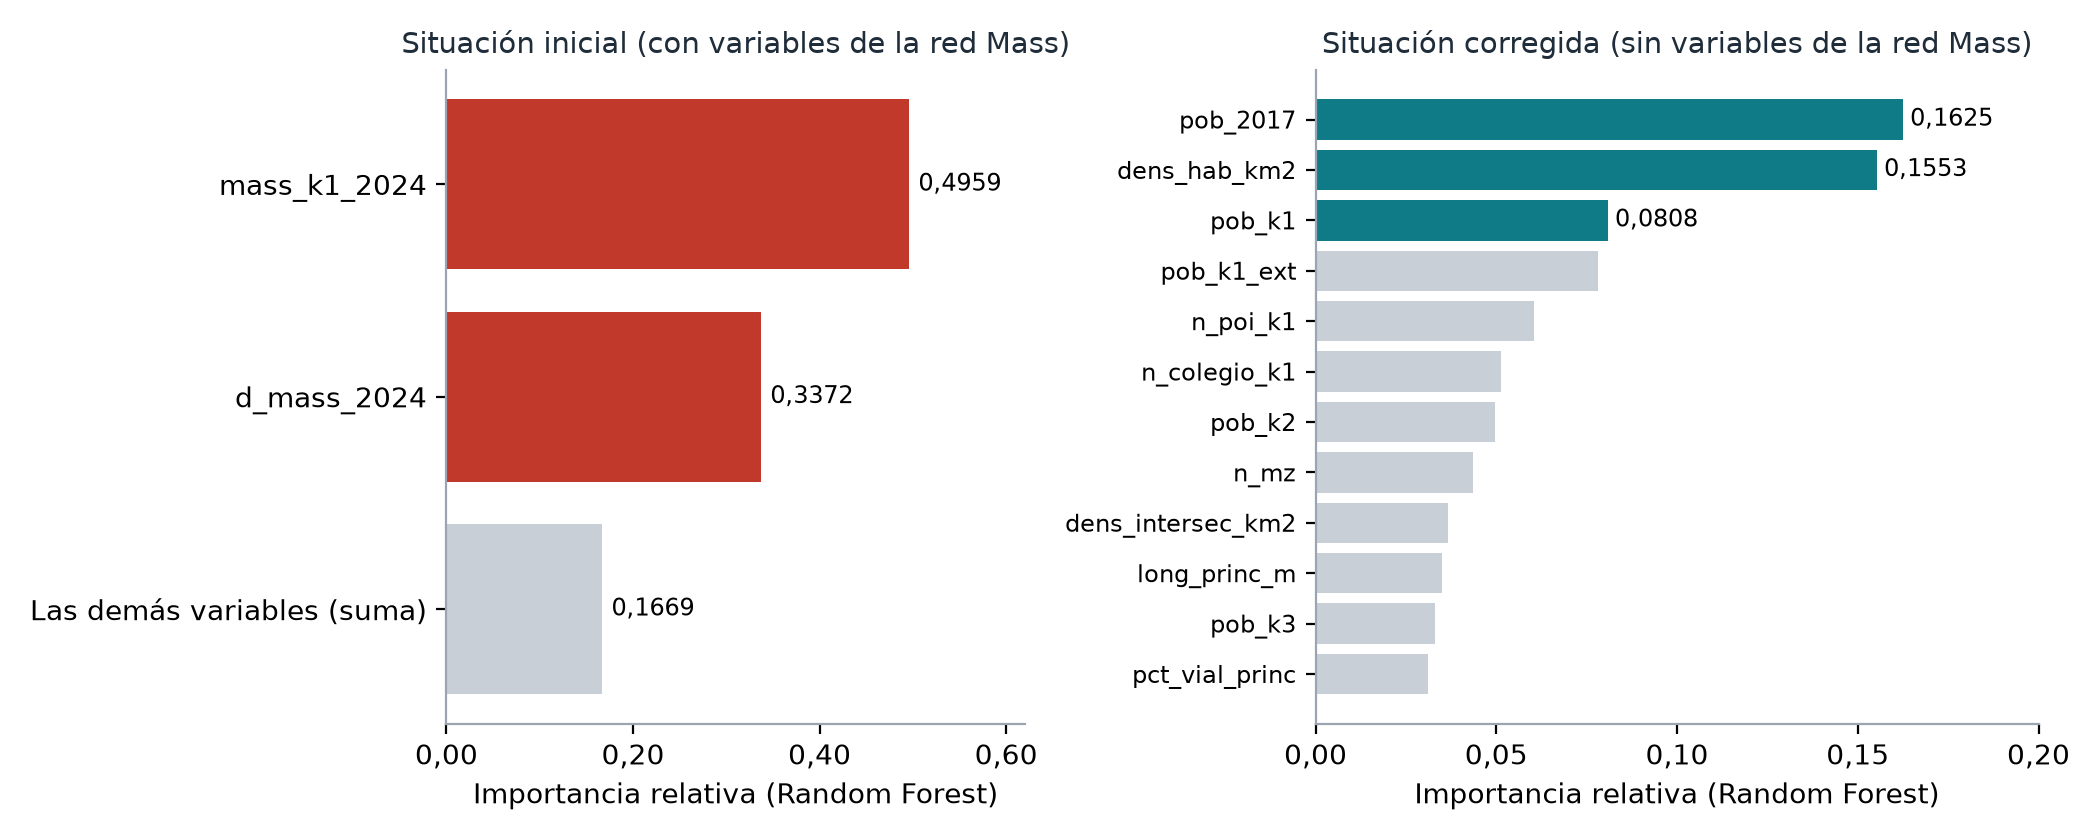
\includegraphics[width=0.82\textwidth]{figuras/fig_importancia.png}
\caption{Importancia de variables antes y después de excluir las variables derivadas de la red de la cadena. El panel izquierdo reproduce los valores de la primera versión del modelo. Fuente: elaboración propia.}
\label{fig:importancia}
\end{figure*}

\subsection{Validación cruzada espacial}

La Tabla~\ref{tab:cv} y la Figura~\ref{fig:curvas} muestran los resultados. Los cuatro modelos superan ampliamente el azar. Random Forest obtiene el mayor ROC-AUC y XGBoost y el ensamble los mayores PR-AUC, con diferencias menores que la variación entre semillas. Al restringir la evaluación a las celdas viables, el ROC-AUC desciende a 0,77--0,79: las 2\,376 celdas no viables, 1\,120 de ellas sin población censal, son negativos fáciles de discriminar y elevan la cifra global (la tasa de eventos es 9,0\,\% entre las viables y 3,3\,\% en el total).

\begin{table}[t]
\centering
\caption{Validación cruzada espacial (52 bloques, cinco pliegues). Media $\pm$ DE de diez semillas; la regresión logística es determinista.}
\label{tab:cv}
\footnotesize
\setlength{\tabcolsep}{3pt}
\begin{tabular}{lccc}
\toprule
Modelo & ROC (3\,717) & ROC (1\,341 viables) & PR (3\,717) \\
\midrule
Reg. logística & 0,865 & 0,733 & 0,202 \\
Random Forest & $0{,}929\pm0{,}001$ & $0{,}793\pm0{,}001$ & $0{,}232\pm0{,}003$ \\
XGBoost & $0{,}922\pm0{,}001$ & $0{,}774\pm0{,}003$ & $0{,}249\pm0{,}008$ \\
Ensamble & $0{,}917\pm0{,}000$ & $0{,}765\pm0{,}001$ & $0{,}255\pm0{,}003$ \\
\bottomrule
\end{tabular}
\end{table}

\begin{figure*}[t]
\centering
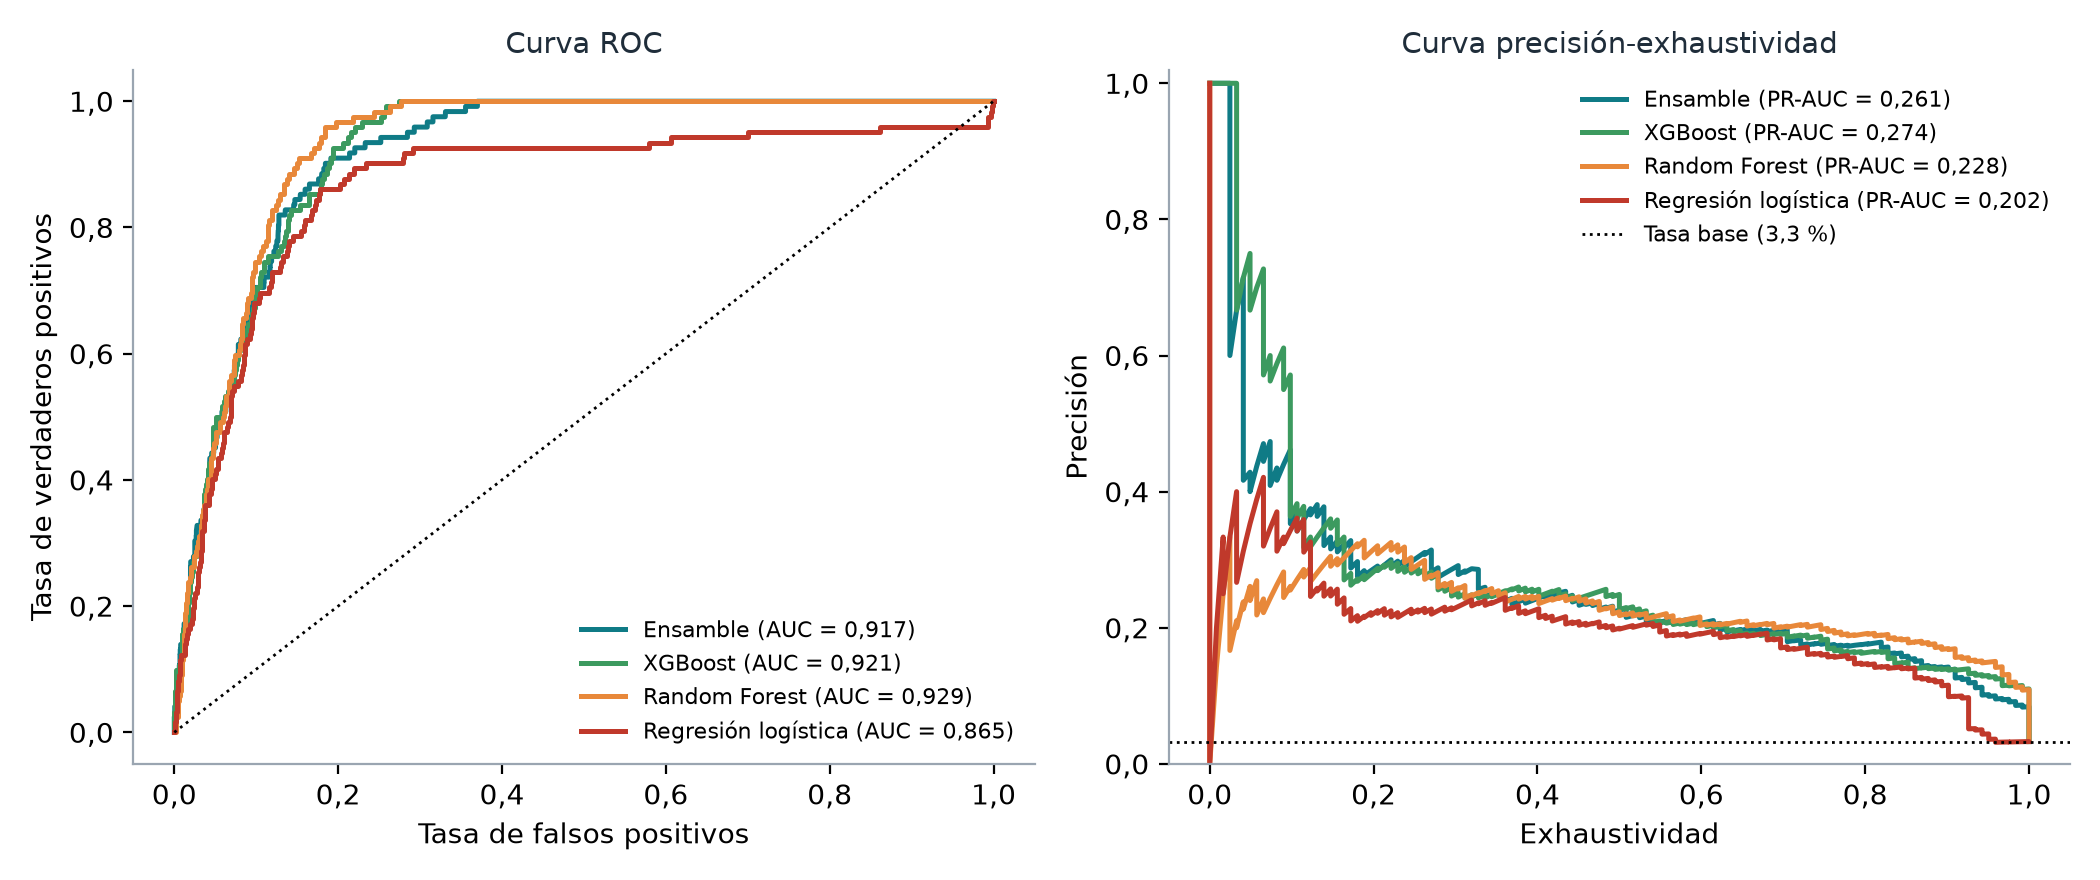
\includegraphics[width=0.82\textwidth]{figuras/fig_curvas_cv.png}
\caption{Curvas ROC y de precisión-exhaustividad bajo validación cruzada espacial (semilla 42). Fuente: elaboración propia.}
\label{fig:curvas}
\end{figure*}

\subsection{Backtesting temporal}

La Tabla~\ref{tab:bt} y la Figura~\ref{fig:lift} presentan el desempeño contra las 39 aperturas reales. El ensamble obtiene los mejores resultados puntuales: ROC-AUC de $0{,}808\pm0{,}002$ y lift de $4{,}29\pm0{,}22$ en diez semillas (4,91 con la semilla 42 del pipeline, IC 95\,\%: 3,02--6,22), y ubica en promedio 3,5 aciertos entre las 20 primeras celdas. Todos los lifts por semilla superan el umbral de 3 (mínimo 3,87). El ensamble supera a los tres criterios univariados, aunque la ventaja sobre el mejor de ellos (población alcanzable, lift 3,10) no es significativa.

\begin{table*}[t]
\centering
\caption{Backtesting temporal sobre 1\,259 celdas candidatas y 39 aperturas reales (2025--2026). Media $\pm$ desviación estándar de diez semillas.}
\label{tab:bt}
\small
\begin{tabular}{lcccc}
\toprule
Modelo & ROC-AUC & PR-AUC & Lift@10\,\% & Aciertos Top-20 \\
\midrule
\multicolumn{5}{l}{\textit{Criterios univariados}} \\
Densidad poblacional & 0,787 & 0,080 & 2,07 & 1 \\
Población alcanzable & 0,754 & 0,092 & 3,10 & 3 \\
POIs de flujo & 0,683 & 0,061 & 2,32 & 1 \\
\midrule
\multicolumn{5}{l}{\textit{Modelos}} \\
Regresión logística & 0,792 & 0,089 & 3,10 & 1 \\
Random Forest & $0{,}790\pm0{,}004$ & $0{,}099\pm0{,}004$ & $3{,}59\pm0{,}26$ & $2{,}0\pm0{,}0$ \\
XGBoost & $0{,}793\pm0{,}005$ & $0{,}112\pm0{,}007$ & $3{,}98\pm0{,}43$ & $3{,}5\pm0{,}8$ \\
Ensamble & $\mathbf{0{,}808\pm0{,}002}$ & $\mathbf{0{,}121\pm0{,}006}$ & $\mathbf{4{,}29\pm0{,}22}$ & $\mathbf{3{,}5\pm0{,}5}$ \\
\bottomrule
\end{tabular}
\end{table*}

\begin{figure}[t]
\centering
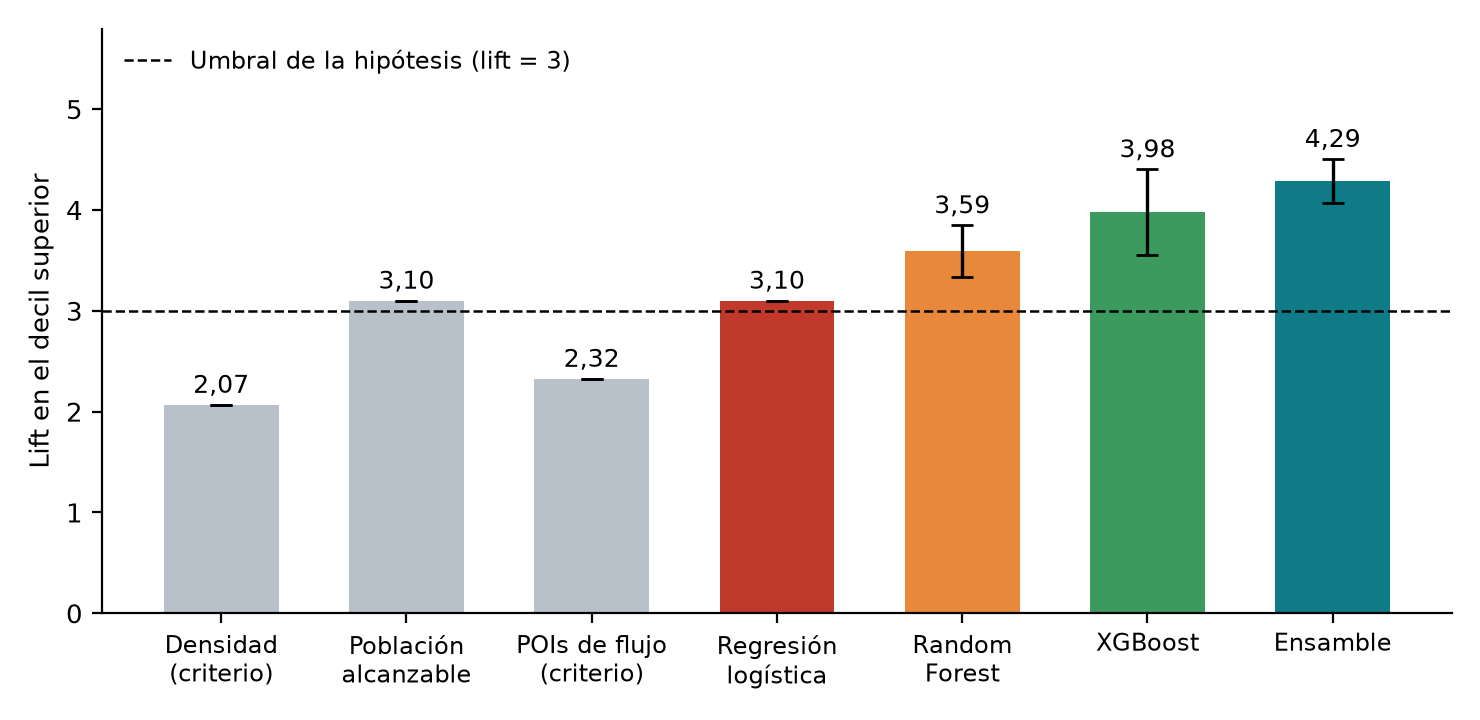
\includegraphics[width=\linewidth]{figuras/fig_lift_backtesting.png}
\caption{Lift en el decil superior del backtesting. Las barras de error son la desviación estándar de diez semillas. Fuente: elaboración propia.}
\label{fig:lift}
\end{figure}

\subsection{Contrastación de la hipótesis}

La Tabla~\ref{tab:hip} evalúa cada condición con el criterio preestablecido. El lift supera el umbral en todas las semillas; el ROC-AUC bajo validación espacial supera 0,85 al evaluar las 3\,717 celdas, pero no al restringirse a las viables (0,766); y la superioridad sobre el mejor criterio univariado se cumple en la estimación puntual (+1,81 puntos de lift, +58,3\,\%), con un intervalo de confianza que incluye el cero. Con 39 eventos positivos, el backtesting carece de potencia para distinguir esa diferencia del azar. La ventaja sobre el criterio de densidad poblacional sí es significativa (+2,84; IC 95\,\%: 0,47--4,28). La hipótesis se sostiene según los criterios preestablecidos, con la salvedad de que la capacidad de discriminar entre ubicaciones comparables es moderada y no alcanza el umbral de 0,85.

\begin{table*}[t]
\centering
\caption{Contrastación de la hipótesis operativa.}
\label{tab:hip}
\small
\begin{tabular}{p{1.9cm}p{4.1cm}p{1.9cm}p{4.1cm}p{3.3cm}}
\toprule
Tipo & Condición (criterio) & IC 95\,\% & Resultado & Estado \\
\midrule
Hipótesis & ROC-AUC bajo validación espacial ($>0{,}85$) & -- & 0,917 (3\,717 celdas); 0,766 (1\,341 viables) & Cumplida; no se mantiene en celdas viables \\
Hipótesis & Lift@10\,\% ($\geq3$) & 3,02--6,22 & 4,91 (semilla 42); $4{,}29\pm0{,}22$ & Confirmada \\
Hipótesis & Lift superior al mejor criterio univariado ($>3{,}10$) & $-0{,}30$--3,56 & +1,81 (+58,3\,\%) & Puntual; no significativa \\
Adicional & PR-AUC frente al mejor criterio ($>0{,}092$) & $-0{,}047$--0,120 & +0,025 (+27,1\,\%) & Puntual; no significativa \\
Adicional & Lift frente a densidad ($>2{,}07$) & 0,47--4,28 & +2,84 & Confirmada \\
\bottomrule
\end{tabular}
\end{table*}

\subsection{Robustez}

Cinco análisis complementarios respaldan los resultados. (i) \textit{Fuga temporal:} con los predictores de OpenStreetMap de 2026 sin filtrar, el ensamble alcanzaba un lift de 3,87 y un ROC-AUC de 0,793; al excluir los locales de la cadena y reconstruir las capas al 31-12-2024 alcanza 4,91 y 0,809, de modo que la métrica limpia no es inferior. (ii) \textit{Autocorrelación espacial:} la variable objetivo tiene un I de Moran de 0,059 ($p=0{,}001$); la partición aleatoria sobreestima el ROC-AUC del ensamble (0,934 frente a 0,917 con bloques), lo que respalda la validación espacial. (iii) \textit{Multicolinealidad:} 11 de 35 predictores evaluados presentan VIF mayor que 10, sobre todo pares absoluto y por km$^2$; los árboles lo toleran y la regresión logística está regularizada. (iv) \textit{Área de aplicabilidad} \citep{meyer2021}: el 93,7\,\% de las celdas y el 94\,\% del Top-50 caen dentro. (v) \textit{Estabilidad entre pliegues:} ROC-AUC del ensamble de $0{,}925\pm0{,}052$, con entre 7 y 59 positivos por pliegue.

\subsection{Pesos elicitados y sensibilidad del ranking}

Los diez propietarios alcanzaron consistencia aceptable (razón de consistencia promedio de 0,052, máximo 0,092; tres requirieron una segunda ronda). La demanda alcanzable domina los criterios (37,7\,\%), seguida de la amenaza del retail moderno (26,1\,\%), el perfil de sitio (25,4\,\%) y la competencia instalada (10,8\,\%). Los comerciantes penalizan la cercanía de las cadenas mucho menos de lo asumido inicialmente (Tabla~\ref{tab:ahp}); con los pesos elicitados el ranking se mantiene robusto frente a los provisionales (rho de Spearman de 0,943; 80\,\% de coincidencia en el Top-10 y en el Top-20).

\begin{table}[t]
\centering
\caption{Parámetros del score: valores provisionales y elicitados.}
\label{tab:ahp}
\footnotesize
\begin{tabular}{lccc}
\toprule
Parámetro & Provisional & Elicitado & Variación \\
\midrule
Peso del perfil ($w$) & 0,450 & 0,344 & $-$23,6\,\% \\
Penalización ($\pi$) & 0,600 & 0,261 & $-$56,5\,\% \\
Radio de amenaza ($R$) & 800\,m & 750\,m & $-$6,3\,\% \\
\bottomrule
\end{tabular}
\end{table}

Al variar $\pm20$\,\% cada parámetro, el peso del perfil, la penalización y el umbral poblacional conservan el 100\,\% del Top-10. El radio de amenaza es el único elemento crítico: conserva entre 80\,\% y 100\,\% dentro de $\pm15$\,\% (638 a 863\,m), pero cae a 40\,\% con $-20\%$ y a 50\,\% con $+20\%$. El ranking cumple el criterio de 70\,\% en los cuatro parámetros dentro de una banda de $\pm15$\,\%.

\subsection{Distribución territorial y simulación económica}

Las oportunidades más altas no se ubican en el centro, sino en un anillo de periferia densa: Miraflores, Jacobo Hunter, Socabaya y Cerro Colorado concentran 33 de las 50 mejores ubicaciones (9, 9, 8 y 7, respectivamente), seguidos de Cayma (6) y Paucarpata (3). El distrito de Arequipa no aporta ninguna. Para una celda representativa de Jacobo Hunter (cuarta posición, score 0,970; 7\,846 habitantes a 500\,m y 65 bodegas estimadas), el simulador estima una cuota de mercado de 3,29\,\%, ventas de S/\,46\,422 mensuales, un margen bruto de S/\,10\,213 y una recuperación de la inversión en 15,7 meses, dentro del rango observado del formato (S/\,30\,000 a 80\,000 mensuales). Sin la estimación de la oferta informal, la misma celda arrojaba una cuota de 100\,\%, ventas de S/\,1\,412\,280 y una recuperación de medio mes, cifras indefendibles.

\subsection{Usabilidad y aceptación}

En el conjunto de los 15 participantes el SUS promedió 77,83 (DE 7,19; mediana 77,5; rango 65--90; IC 95\,\%: 73,85--81,81; alfa de Cronbach 0,744), significativamente por encima del promedio histórico de 68 puntos ($t(14)=5{,}298$; $p<0{,}001$; $d=1{,}368$); el 86,7\,\% valoró la usabilidad como buena o excelente. Frente al criterio de 75, en cambio, la diferencia no es significativa ($t(14)=1{,}527$; $p=0{,}149$). El TAM global fue de 4,13 (utilidad 4,16; facilidad 4,09; intención 4,16; alfa de 0,71), y ninguna dimensión supera el criterio de 4,0 con significancia estadística ($p$ entre 0,110 y 0,340).

La Tabla~\ref{tab:sus} muestra los resultados por perfil. No se detectaron diferencias significativas entre perfiles (Kruskal-Wallis, $H=5{,}332$; $p=0{,}149$), resultado esperable con subgrupos de tres a cinco personas. Sin embargo, los propietarios de minimarket, que son los usuarios finales del sistema, quedaron por debajo de ambos umbrales.

\begin{table*}[t]
\centering
\caption{Usabilidad (SUS, 0--100) y aceptación tecnológica (TAM, 1--5) por perfil.}
\label{tab:sus}
\small
\begin{tabular}{lcccccc}
\toprule
Perfil & $n$ & SUS & Utilidad & Facilidad & Intención & TAM global \\
\midrule
Corredores inmobiliarios & 4 & 84,38 & 4,50 & 4,38 & 4,58 & 4,49 \\
Estudiantes de posgrado & 3 & 77,50 & 4,11 & 4,11 & 4,11 & 4,11 \\
Docentes del área & 3 & 75,83 & 4,06 & 4,06 & 4,11 & 4,07 \\
Propietarios de minimarket & 5 & 74,00 & 3,97 & 3,87 & 3,87 & 3,90 \\
\midrule
Global (promedio ponderado) & 15 & 77,83 & 4,16 & 4,09 & 4,16 & 4,13 \\
\bottomrule
\end{tabular}
\end{table*}

%% ---------------------------------------------------------------------
\section{Discusión}

\textbf{Interpretación.} El modelo aprende que la apertura de una cadena profesional responde sobre todo a la demanda poblacional local, un perfil consistente con el concepto de umbral mínimo de demanda de la teoría del lugar central \citep{christaller1966}. Esto sustenta la preferencia revelada como sustituto de las ventas, pero también define su alcance: el sistema identifica zonas de demanda validada por el mercado, no zonas protegidas de la competencia. En el backtesting, 38 de las 50 celdas mejor puntuadas al corte de 2024 (76\,\%) registraron una apertura de la cadena a menos de 750\,m durante 2025--2026, frente al 35\,\% de las celdas viables. Para un minimarket independiente sin central de compras esa cercanía es una amenaza, y por eso el score la penaliza y la aplicación advierte las celdas con alta probabilidad de entrada.

\textbf{Criterio de decisión.} El panel de propietarios asigna a la competencia instalada el menor peso (10,8\,\%), en línea con la lógica de aglomeración comercial \citep{zhang2025}, y a la amenaza de las cadenas un peso equivalente al del perfil de sitio. Que el radio de amenaza sea el único parámetro crítico justifica haberlo elicitado empíricamente y no asumido.

\textbf{Comparación con la literatura.} Las exactitudes de 0,900 y 0,922 de \citet{zhao2025}, o de aproximadamente 0,76 de \citet{ou2026}, no son directamente comparables con los ROC-AUC reportados aquí: miden otra métrica y ninguno de los estudios revisados declara validación en bloques espaciales, cuyo efecto puede ser considerable \citep{ploton2020,kumar2025}.

\textbf{Lecciones de validación.} Tres hallazgos conviene destacar. Primero, una variable derivada de la propia red de la cadena produjo un modelo que aparentaba ser bueno y optimizaba en dirección contraria a la lógica del negocio; el backtesting con predictores al corte de 2024 fue lo que lo reveló. Segundo, la cifra de validación espacial global (0,917) sobrestima la capacidad de ordenar ubicaciones comparables (0,766), coherente con el 0,808 del backtesting. Tercero, una sola semilla puede favorecer al ensamble: el lift de 4,91 es el extremo alto de un rango de 3,87 a 4,65 en diez semillas.

\textbf{Limitaciones.} (i) Solo hay 39 eventos positivos y una ventana de dos años, por lo que las métricas del extremo superior del ranking tienen alta varianza. (ii) La variable objetivo representa las decisiones de una única cadena e indica que un emplazamiento opera, no que sea rentable. (iii) La cobertura de OpenStreetMap en comercios es parcial y la competencia informal es una estimación. (iv) La población proviene del Censo 2017; el Censo 2025 \citep{inei2026} registra 13,1\,\% más habitantes en el área metropolitana, por lo que se asume que la distribución espacial relativa se mantiene. (v) La proximidad se mide con distancia euclidiana, sin enrutamiento peatonal. (vi) Los criterios de usabilidad y aceptación se cumplen en la estimación puntual pero sin significancia estadística con 15 participantes, y los propietarios de minimarket, usuarios finales, puntuaron por debajo de ambos umbrales (SUS 74,00; TAM 3,90) con una muestra de cinco personas; no puede afirmarse que la aceptación se mantenga en esa población. (vii) No se contrastó la significancia de las diferencias entre modelos. (viii) El estudio abarca una sola ciudad.

%% ---------------------------------------------------------------------
\section{Conclusiones}

Es posible construir y validar, con fuentes exclusivamente públicas, un sistema de soporte a la decisión para localizar minimarkets independientes sin acceder a series de ventas. El ensamble de modelos concentró en su decil superior 4,29 veces más aperturas reales que un decil aleatorio en el backtesting temporal (rango 3,87--4,65 en diez semillas), con un ROC-AUC de 0,917 bajo validación espacial y de 0,808 en el backtesting. La hipótesis se sostiene según los criterios preestablecidos, pero la capacidad de discriminar entre ubicaciones comparables es moderada (ROC-AUC de 0,77 a 0,81) y la ventaja sobre el mejor criterio univariado no es estadísticamente significativa. El sistema alcanzó los criterios de usabilidad y aceptación en el conjunto de usuarios, no así entre los propietarios de minimarket. Como trabajo futuro se propone ampliar la ventana histórica, incorporar otras cadenas como evidencia de preferencia revelada, replicar la evaluación con una muestra mayor de propietarios, incorporar enrutamiento peatonal y transferir el diseño a otras ciudades peruanas, dado que las cuatro fuentes integradas tienen cobertura nacional.

\section*{Disponibilidad de datos y código}
El código, los datos derivados y las instrucciones para reproducir los resultados están disponibles en \url{https://github.com/PaoloRivera/sigret-aqp}. Los datos de OpenStreetMap se distribuyen bajo la licencia ODbL.

%% ---------------------------------------------------------------------
\balance
\begin{thebibliography}{99}
\footnotesize
\setlength{\parindent}{-0.45cm}\setlength{\leftskip}{0.45cm}

\bibitem[Brodsky(2018)]{brodsky2018} Brodsky, I. (2018). H3: Uber's hexagonal hierarchical spatial index. \textit{Uber Engineering Blog}. \url{https://www.uber.com/en-HR/blog/h3/}

\bibitem[Breiman(2001)]{breiman2001} Breiman, L. (2001). Random forests. \textit{Machine Learning, 45}(1), 5--32. \url{https://doi.org/10.1023/A:1010933404324}

\bibitem[Brooke(1996)]{brooke1996} Brooke, J. (1996). SUS: A ``quick and dirty'' usability scale. En P. W. Jordan, B. Thomas, B. A. Weerdmeester y I. L. McClelland (Eds.), \textit{Usability evaluation in industry} (pp. 189--194). Taylor \& Francis.

\bibitem[Chen y Guestrin(2016)]{chen2016} Chen, T., y Guestrin, C. (2016). XGBoost: A scalable tree boosting system. En \textit{Proceedings of the 22nd ACM SIGKDD International Conference on Knowledge Discovery and Data Mining} (pp. 785--794). ACM. \url{https://doi.org/10.1145/2939672.2939785}

\bibitem[Christaller(1966)]{christaller1966} Christaller, W. (1966). \textit{Central places in southern Germany} (C. W. Baskin, Trad.). Prentice-Hall. (Obra original publicada en 1933)

\bibitem[Davis(1989)]{davis1989} Davis, F. D. (1989). Perceived usefulness, perceived ease of use, and user acceptance of information technology. \textit{MIS Quarterly, 13}(3), 319--340. \url{https://doi.org/10.2307/249008}

\bibitem[{Deloitte}(2025)]{deloitte2025} Deloitte. (2025). \textit{El avance del hard discount: evolución y perspectivas hacia 2030}. \url{https://www.deloitte.com/latam/es/services/consulting/perspectives/el-avance-del-hard-discount--evolucion-y-perspectivas-hacia-2030.html}

\bibitem[D'Silva et~al.(2018)]{dsilva2018} D'Silva, K., Jayarajah, K., Noulas, A., Mascolo, C., y Misra, A. (2018). The role of urban mobility in retail business survival. \textit{Proceedings of the ACM on Interactive, Mobile, Wearable and Ubiquitous Technologies, 2}(3), Artículo 100. \url{https://doi.org/10.1145/3264910}

\bibitem[He y Garcia(2009)]{he2009} He, H., y Garcia, E. A. (2009). Learning from imbalanced data. \textit{IEEE Transactions on Knowledge and Data Engineering, 21}(9), 1263--1284. \url{https://doi.org/10.1109/TKDE.2008.239}

\bibitem[Hu et~al.(2025)]{hu2025} Hu, H., Tan, D., Thaichon, P., Wang, B., y Zhu, Z. (2025). Grid-based market sales forecasting for retail businesses using automated machine learning and geospatial intelligence. \textit{Expert Systems with Applications, 284}, 127869. \url{https://doi.org/10.1016/j.eswa.2025.127869}

\bibitem[Huff(1964)]{huff1964} Huff, D. L. (1964). Defining and estimating a trading area. \textit{Journal of Marketing, 28}(3), 34--38. \url{https://doi.org/10.1177/002224296402800307}

\bibitem[{INEI}(2018)]{inei2018} Instituto Nacional de Estadística e Informática. (2018). \textit{Censos Nacionales 2017: XII de Población, VII de Vivienda y III de Comunidades Indígenas. Arequipa: Resultados definitivos (Tomo I)}. INEI.

\bibitem[{INEI}(2024)]{inei2024} Instituto Nacional de Estadística e Informática. (2024). \textit{Demografía empresarial en el Perú: III trimestre de 2024} (Informe Técnico N.° 04). INEI. \url{https://www.inei.gob.pe/media/MenuRecursivo/boletines/demografia_empresarial_3t24.pdf}

\bibitem[{INEI}(2026)]{inei2026} Instituto Nacional de Estadística e Informática. (2026). \textit{Censos Nacionales 2025: XIII de Población, VIII de Vivienda y IV de Comunidades Indígenas -- Plataforma de resultados}. \url{https://censos2025.inei.gob.pe/resultados}

\bibitem[Karamshuk et~al.(2013)]{karamshuk2013} Karamshuk, D., Noulas, A., Scellato, S., Nicosia, V., y Mascolo, C. (2013). Geo-spotting: Mining online location-based services for optimal retail store placement. En \textit{Proceedings of the 19th ACM SIGKDD International Conference on Knowledge Discovery and Data Mining} (pp. 793--801). ACM. \url{https://doi.org/10.1145/2487575.2487616}

\bibitem[Kmoch et~al.(2022)]{kmoch2022} Kmoch, A., Vasilyev, I., Virro, H., y Uuemaa, E. (2022). Area and shape distortions in open-source discrete global grid systems. \textit{Big Earth Data, 6}(3), 256--275. \url{https://doi.org/10.1080/20964471.2022.2094926}

\bibitem[Kumar et~al.(2025)]{kumar2025} Kumar, C., Walton, G., Santi, P., y Luza, C. (2025). Random cross-validation produces biased assessment of machine learning performance in regional landslide susceptibility prediction. \textit{Remote Sensing, 17}(2), 213. \url{https://doi.org/10.3390/rs17020213}

\bibitem[Liang et~al.(2020)]{liang2020} Liang, Y., Gao, S., Cai, Y., Foutz, N. Z., y Wu, L. (2020). Calibrating the dynamic Huff model for business analysis using location big data. \textit{Transactions in GIS, 24}(3), 681--703. \url{https://doi.org/10.1111/tgis.12624}

\bibitem[Lu et~al.(2024)]{lu2024} Lu, J., Zheng, X., Nervino, E., Li, Y., Xu, Z., y Xu, Y. (2024). Retail store location screening: A machine learning-based approach. \textit{Journal of Retailing and Consumer Services, 77}, 103620. \url{https://doi.org/10.1016/j.jretconser.2023.103620}

\bibitem[Meyer y Pebesma(2021)]{meyer2021} Meyer, H., y Pebesma, E. (2021). Predicting into unknown space? Estimating the area of applicability of spatial prediction models. \textit{Methods in Ecology and Evolution, 12}(9), 1620--1633. \url{https://doi.org/10.1111/2041-210X.13650}

\bibitem[{Ministerio de la Producción}(2025)]{produce2025} Ministerio de la Producción. (2025). \textit{Caracterización de los negocios del comercio al por menor en el Perú}. Observatorio PRODUCEmpresarial. \url{https://www.producempresarial.pe/wp-content/uploads/2025/03/282-PPT_-Bodegueros_2024_14.03.2025.pdf}

\bibitem[Openshaw(1984)]{openshaw1984} Openshaw, S. (1984). \textit{The modifiable areal unit problem} (Concepts and Techniques in Modern Geography N.º 38). Geo Books.

\bibitem[Ou et~al.(2026)]{ou2026} Ou, T.-Y., Fu, H.-P., y Wu, M.-Z. (2026). Optimize a chain convenience store location prediction model by using MTS-machine learning methodology. \textit{Scientific Reports, 16}, 1056. \url{https://doi.org/10.1038/s41598-025-30650-w}

\bibitem[Peffers et~al.(2007)]{peffers2007} Peffers, K., Tuunanen, T., Rothenberger, M. A., y Chatterjee, S. (2007). A design science research methodology for information systems research. \textit{Journal of Management Information Systems, 24}(3), 45--77. \url{https://doi.org/10.2753/MIS0742-1222240302}

\bibitem[{Perú Retail}(2026)]{peruretail2026} Perú Retail. (2026). \textit{Conoce cuántas tiendas tienen las principales cadenas en Perú y cuánto crecerán en 2026}. \url{https://www.peru-retail.com/cuantas-tiendas-tienen-las-principales-cadenas-en-peru-y-cuanto-creceran-en-2026/}

\bibitem[Ploton et~al.(2020)]{ploton2020} Ploton, P., Mortier, F., Réjou-Méchain, M., Barbier, N., Picard, N., Rossi, V., Dormann, C., Cornu, G., Viennois, G., Bayol, N., Lyapustin, A., Gourlet-Fleury, S., y Pélissier, R. (2020). Spatial validation reveals poor predictive performance of large-scale ecological mapping models. \textit{Nature Communications, 11}, 4540. \url{https://doi.org/10.1038/s41467-020-18321-y}

\bibitem[Roberts et~al.(2017)]{roberts2017} Roberts, D. R., Bahn, V., Ciuti, S., Boyce, M. S., Elith, J., Guillera-Arroita, G., Hauenstein, S., Lahoz-Monfort, J. J., Schröder, B., Thuiller, W., Warton, D. I., Wintle, B. A., Hartig, F., y Dormann, C. F. (2017). Cross-validation strategies for data with temporal, spatial, hierarchical, or phylogenetic structure. \textit{Ecography, 40}(8), 913--929. \url{https://doi.org/10.1111/ecog.02881}

\bibitem[Rossi et~al.(2024)]{rossi2024} Rossi, J. L., Ibazeta Quispe, O., Latorre Asmad, M. R., y Ochoa Pérez, D. V. (2024). \textit{Proceso sistemático para la ubicación de tiendas minoristas en entornos urbanos de Lima} [Trabajo de investigación de maestría, Universidad Peruana de Ciencias Aplicadas]. Repositorio Académico UPC. \url{https://repositorioacademico.upc.edu.pe/handle/10757/675921}

\bibitem[Saaty(1990)]{saaty1990} Saaty, T. L. (1990). How to make a decision: The analytic hierarchy process. \textit{European Journal of Operational Research, 48}(1), 9--26. \url{https://doi.org/10.1016/0377-2217(90)90057-I}

\bibitem[Samuelson(1938)]{samuelson1938} Samuelson, P. A. (1938). A note on the pure theory of consumer's behaviour. \textit{Economica, 5}(17), 61--71. \url{https://doi.org/10.2307/2548836}

\bibitem[Tullis y Stetson(2004)]{tullis2004} Tullis, T. S., y Stetson, J. N. (2004). A comparison of questionnaires for assessing website usability. \textit{Usability Professionals Association Conference}.

\bibitem[Zhang et~al.(2025)]{zhang2025} Zhang, J., Song, J., y Zeng, J. (2025). Toward resilience: Assessing retail location's complex impact mechanism using PLS-SEM aided by machine learning. \textit{Sustainability, 17}(16), 7461. \url{https://doi.org/10.3390/su17167461}

\bibitem[Zhao et~al.(2025)]{zhao2025} Zhao, Z., Chen, G., Duan, J., y Xu, Y. (2025). Site selection analysis and prediction of new retail stores from an urban commercial space perspective: A case study of Luckin Coffee and Starbucks in Shanghai. \textit{ISPRS International Journal of Geo-Information, 14}(6), 217. \url{https://doi.org/10.3390/ijgi14060217}

\bibitem[Zou et~al.(2024)]{zou2024} Zou, J., Zhang, X., Cong, Y., Gao, Z., y Shi, J. (2024). Research and modeling of commercial location selection based on geographic big data and mobile signaling data---A case study of the central urban area of Beijing. \textit{ISPRS International Journal of Geo-Information, 13}(12), 432. \url{https://doi.org/10.3390/ijgi13120432}

\end{thebibliography}

\end{document}
